\documentclass[a4paper]{article}

\usepackage[english]{babel}
\usepackage[utf8x]{inputenc}
\usepackage[T1]{fontenc}
\usepackage[a4paper,top=3cm,bottom=2cm,left=3cm,right=3cm,marginparwidth=1.75cm]{geometry}
\usepackage{amsmath}
\usepackage{graphicx}
\usepackage[colorinlistoftodos]{todonotes}
\usepackage[colorlinks=true, allcolors=blue]{hyperref}
\usepackage{float}
\usepackage{enumerate}
\usepackage{subfig}
\usepackage{ctex}
\usepackage{listings}
\usepackage{xcolor}


\title{Introduction to elgooG Search Engine}
\author{Zhipeng Chen}

\begin{document}
\maketitle

\begin{abstract}
	
	elgooG Search Engine can search the websites of the School of Infomation in Renmin University of China, and present the article which user wants to read.The search engine uses inverted index so that it can present the pretty relevant passage from all websites.
	
\end{abstract}

\section{The function of engine}
	
	\subsection{UI}
	
		The initial interface contains the logo and a text frame. 
		
		\begin{center}
		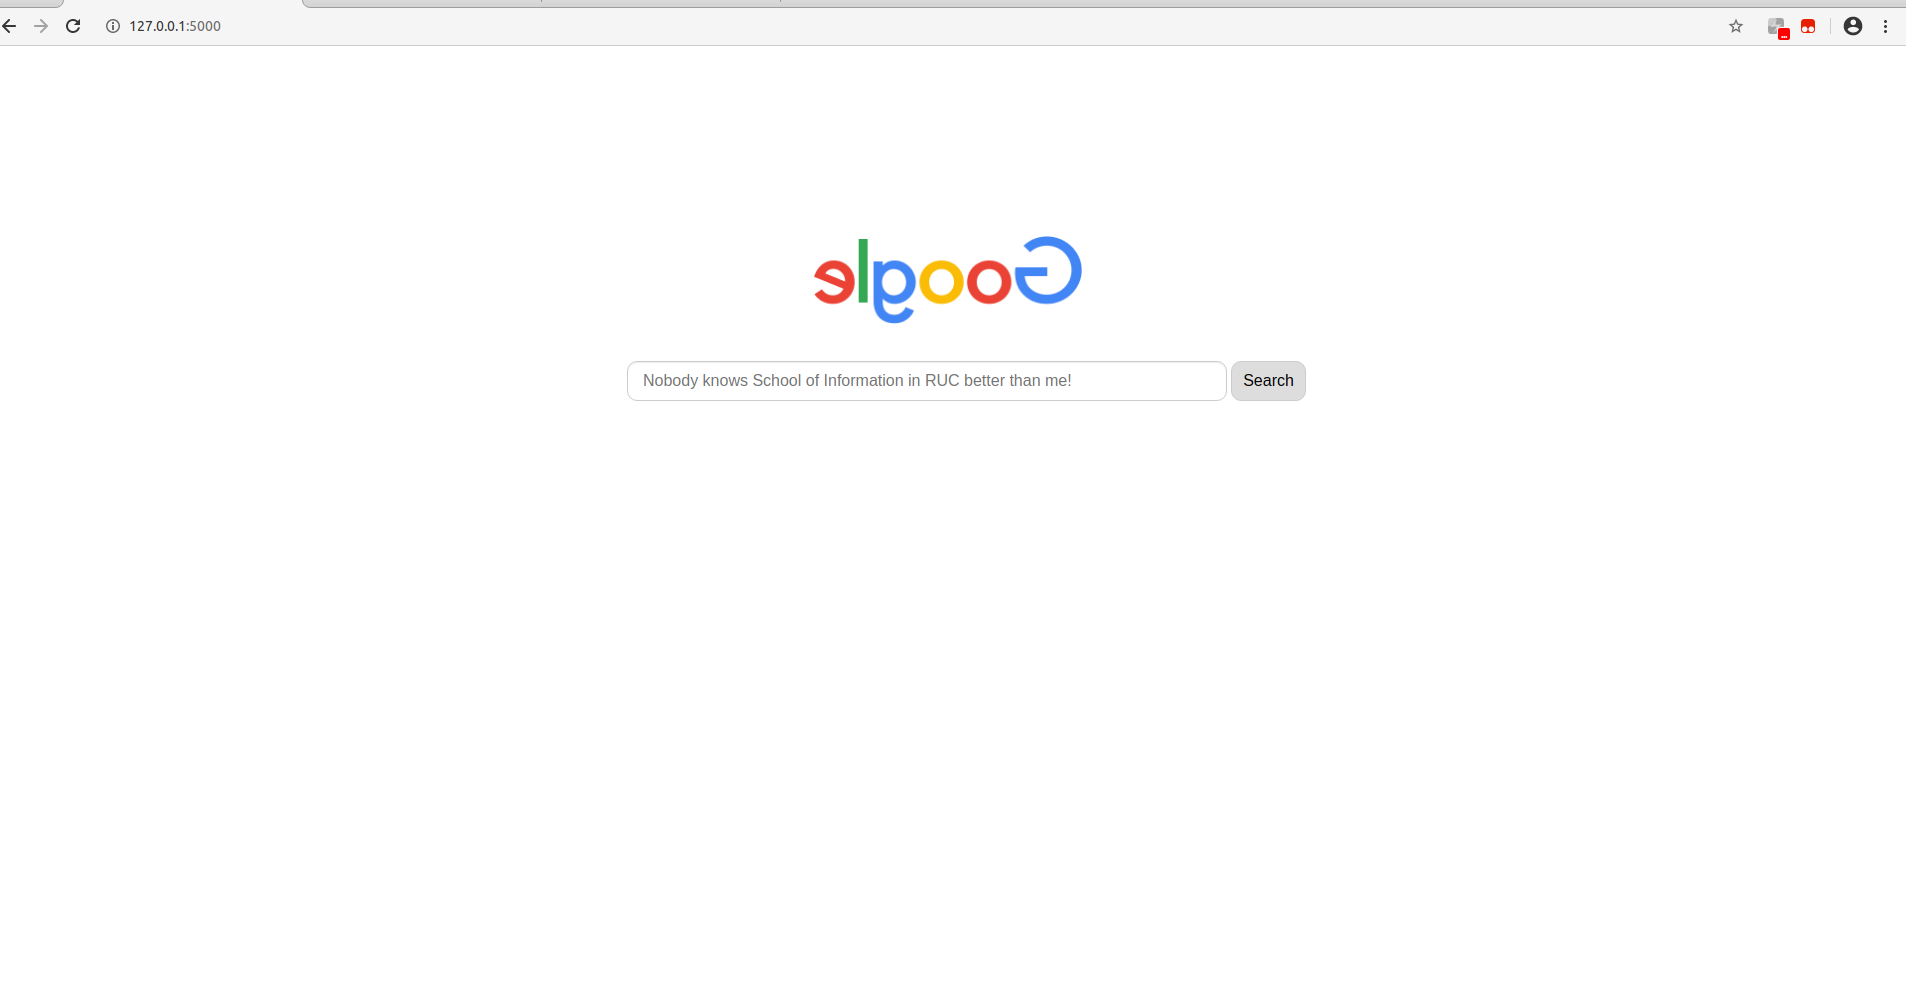
\includegraphics[width=0.6\textwidth, height=0.2\textheight]{UI-1.png}
		\end{center}
		
		When user search something on the engine, it will jump to the interface showing the results.
		
		\begin{center}
		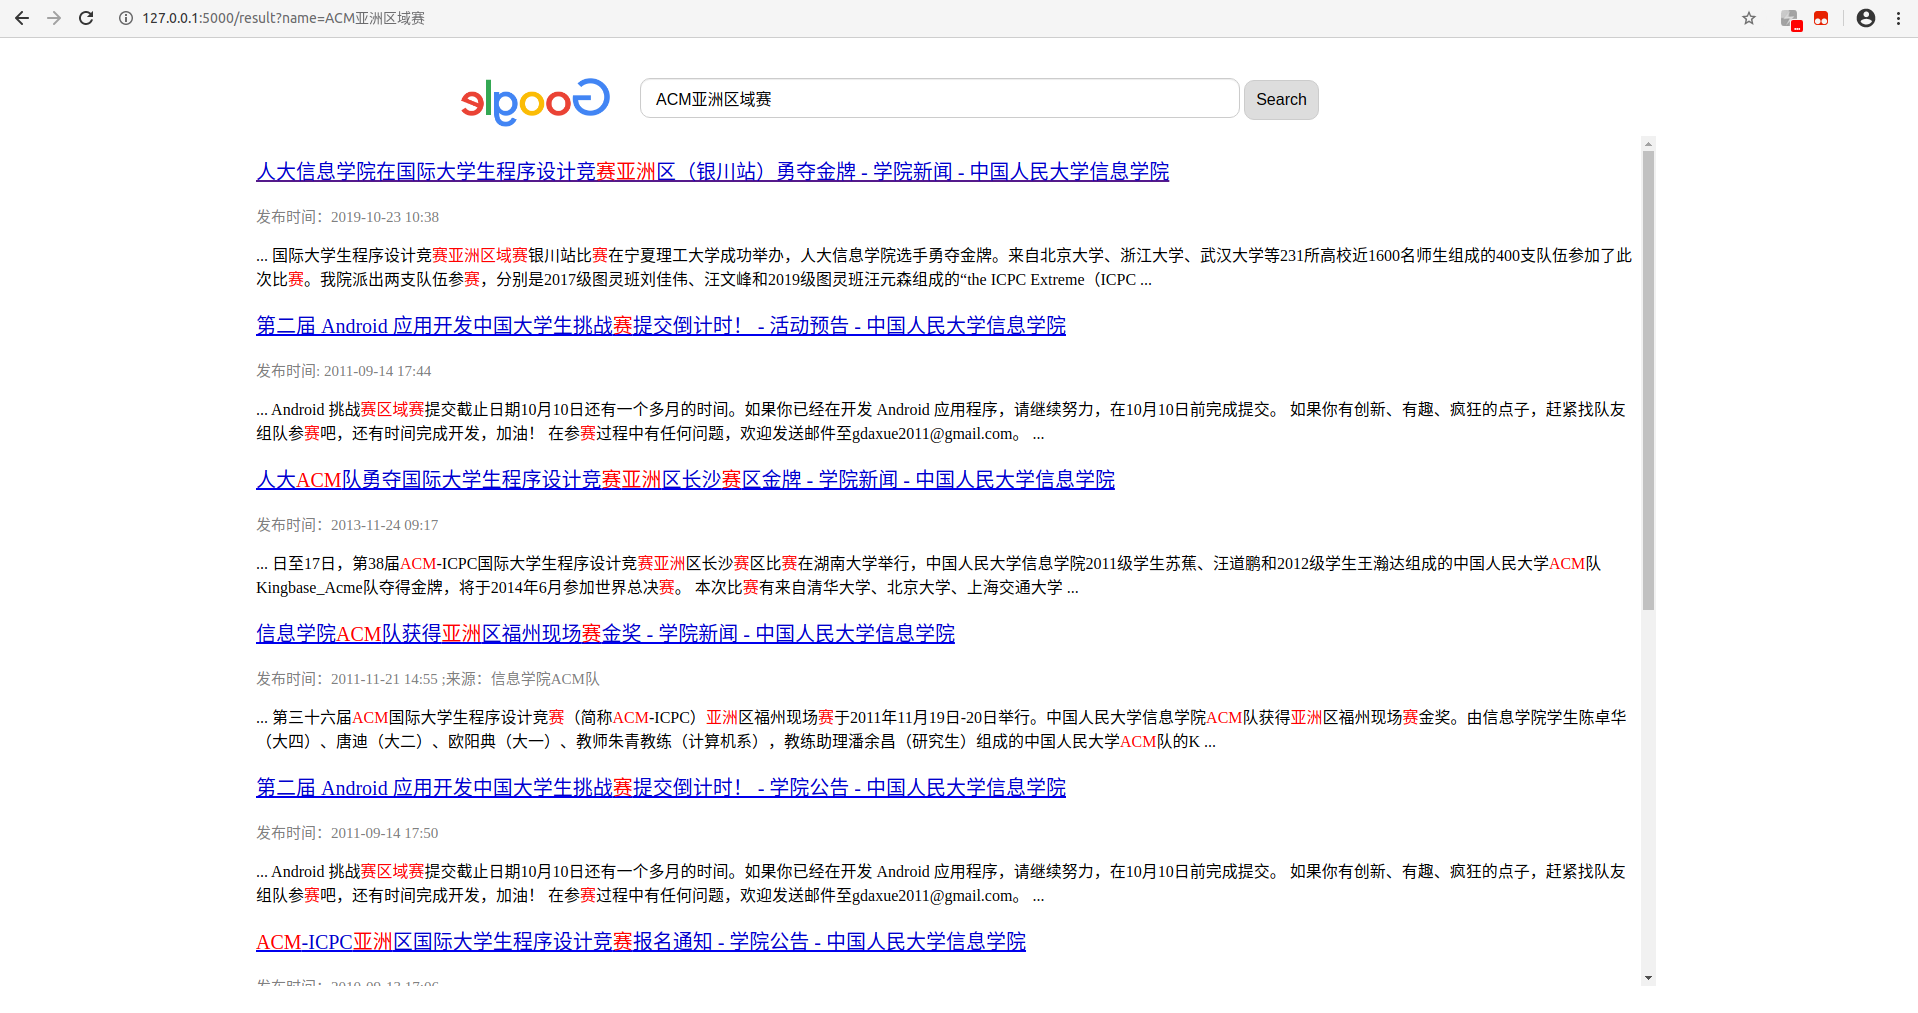
\includegraphics[width=0.6\textwidth, height=0.2\textheight]{UI-2.png}
		\end{center}
	
	\subsection{Function} 
	
		In the initial interface, users can type something into the text frame to search for the relevant passage. The engine will to show the resulte about the question that users asked. Each result contains the title, time, source and a brief instruction for the article(if they exist). The relevant element in the detial of the result will be showed in red.
		
		In the result interface, users can search something different in the text frame. Engine will return the result about the new question.

\section{The way to make engine}
	
	\subsection{Crawler}
		
		In order to get all the websites of the School of Infomation, I use a crawler to download the websites. The crawler is written by C++ programming language. When it reach a website, crawler will search the html document about this website for the urls which haven't been reached. Then the crawler will download the unreaching websites by using the system command 'wget' and make a flag for it. Through the BFS(Breadth First Search), the crawler will download all the websites we need.
	
	\subsection{Normalized and divided}
		
		The code to translate the html document to text is written by python programming language. First, the program will read each document that have been download before. Then, it will find the title, source, time and main body of the article by using BeautifulSoup4(a package in python). Finally, it will save the detial in other documents.
		
		The code to divided the normalized document is written by python programming language. The program will cut the document into some words by using jieba(a package in python), and save the results in other documents. After cutting document, it's convenient to search for the most relevant website.
	
	\subsection{Search for result}
	
		The elgooG uses the inverted index which is the classical model to build a search engine. The process is worked before the search engine start.
		
		After that, the search engine can return the question that users asked. When the engine get a query, it will cut the query into some words by using jieba. Then it will calculate the sorce of each website and return the top 10 website as result. The fomula to calculate the sorce is the one below:
		
		\begin{center}
			
			$Sorce_i = \sum{Value_{i,id}}$
			
			$Value_{i,id} = (1 + \lg(t_{i,id})) * (\lg(\frac{N}{n_{id}}))^{1.75} * (\lg(len_{id}+1))$
			
		\end{center}
		
		The $Sorce_i$ is the sorce of $i$th website; the $Value_{i,id}$ is the value of $id$th word in $i$th website; the $t_{id}$ is the times of the $id$th word appearing in $i$th website; the $N$ is the sum of the words in all website; the $n_{id}$ is the times of the $id$th word appearing in all websites; the $len_{id}$ is the lenght of the $i$th word.
		
		In the words from query, if a word is made by number, it will have higher value. It's value can be calculate by the fomula below:
		
		\begin{center}
			$Value_{i,id} = (1 + \lg(t_{i,id})) * (\lg(\frac{N}{n_{id}}))^{1.75} * (\lg(len_{id}+1)) * (\lg(len_{id} + 1) + 1.6) $
		\end{center}

\section{The skills of programming}
	
	First, a huge project can be divided into some small part. Finishing the small part is easier than finishing the whole project at once. At the smae time, it's also easy to code and debug in the small part of project.
	
	Second, coding with a clear mind. If you don't know what you are doing, you will make many bugs instead of writing correct code.
	
	Third, learning the grammer of new programming language first, if you want to write code through it.

\section{Some examples}
	
	Search for teacher:
	\begin{center}
		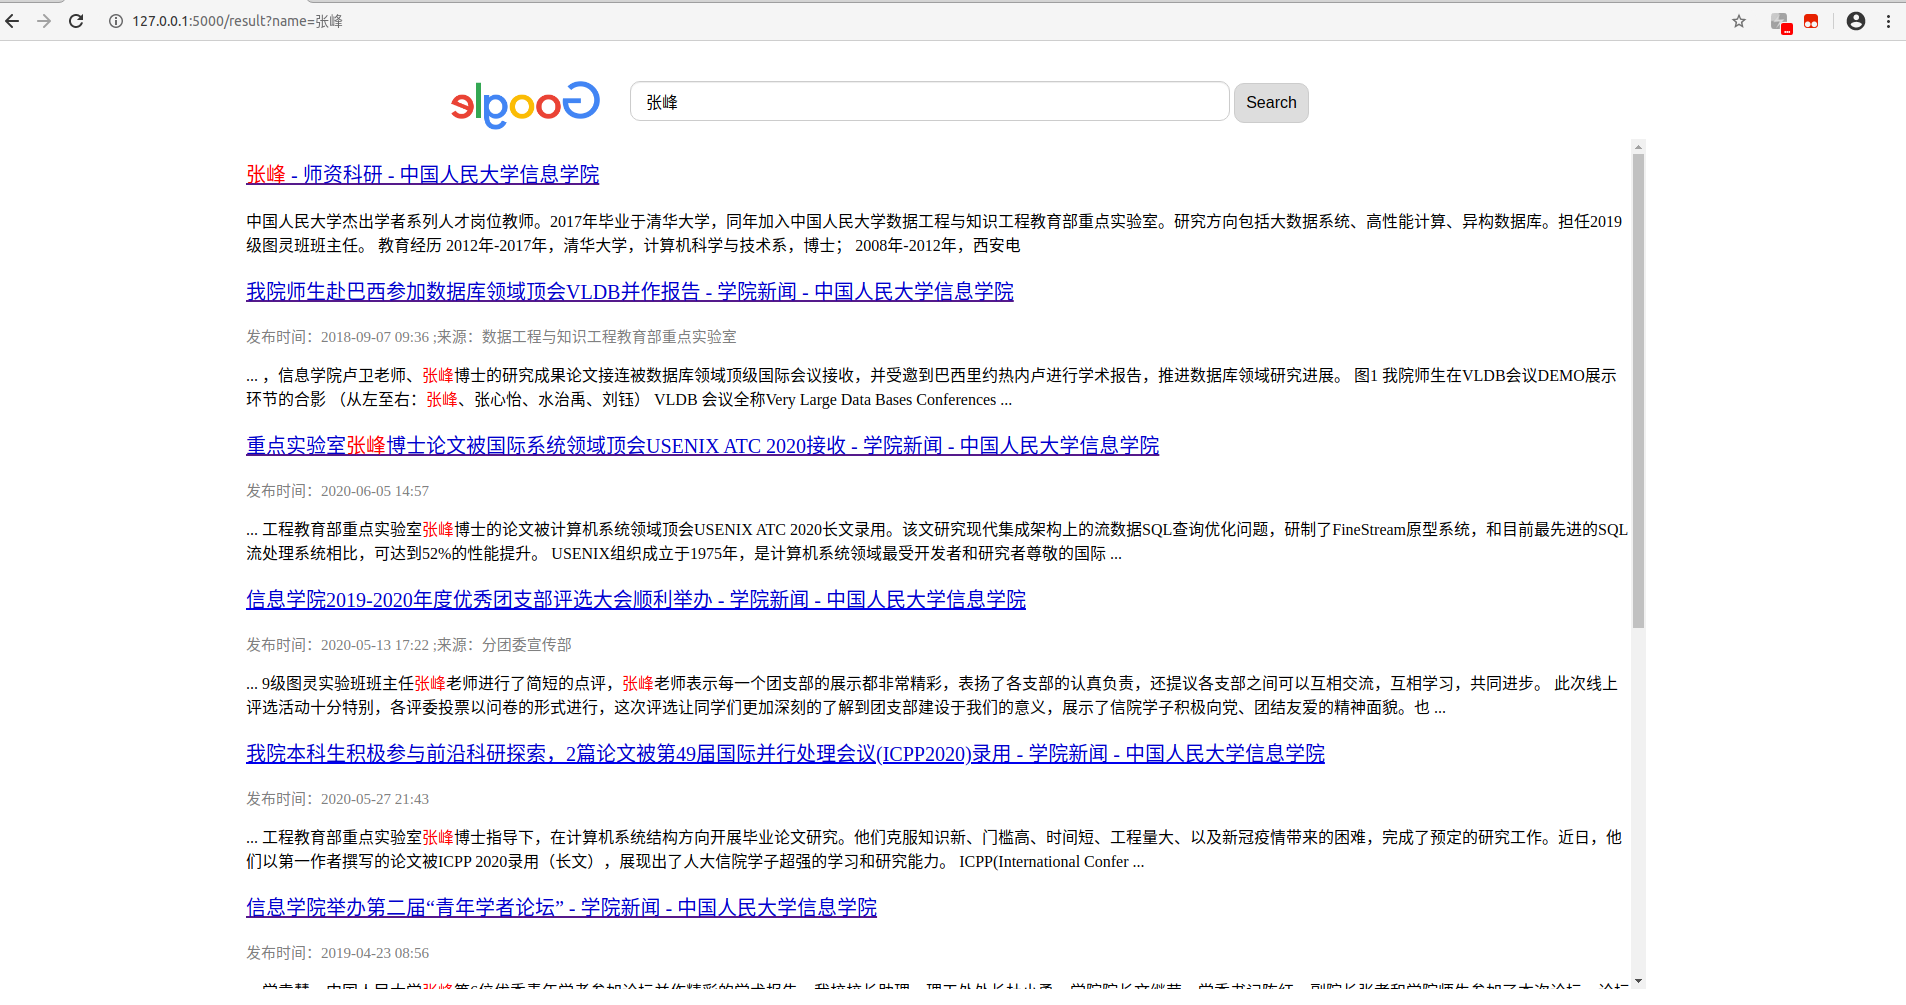
\includegraphics[width=0.6\textwidth, height=0.2\textheight]{zf.png}
	\end{center}
		
	Search for laboratory:
	\begin{center}
		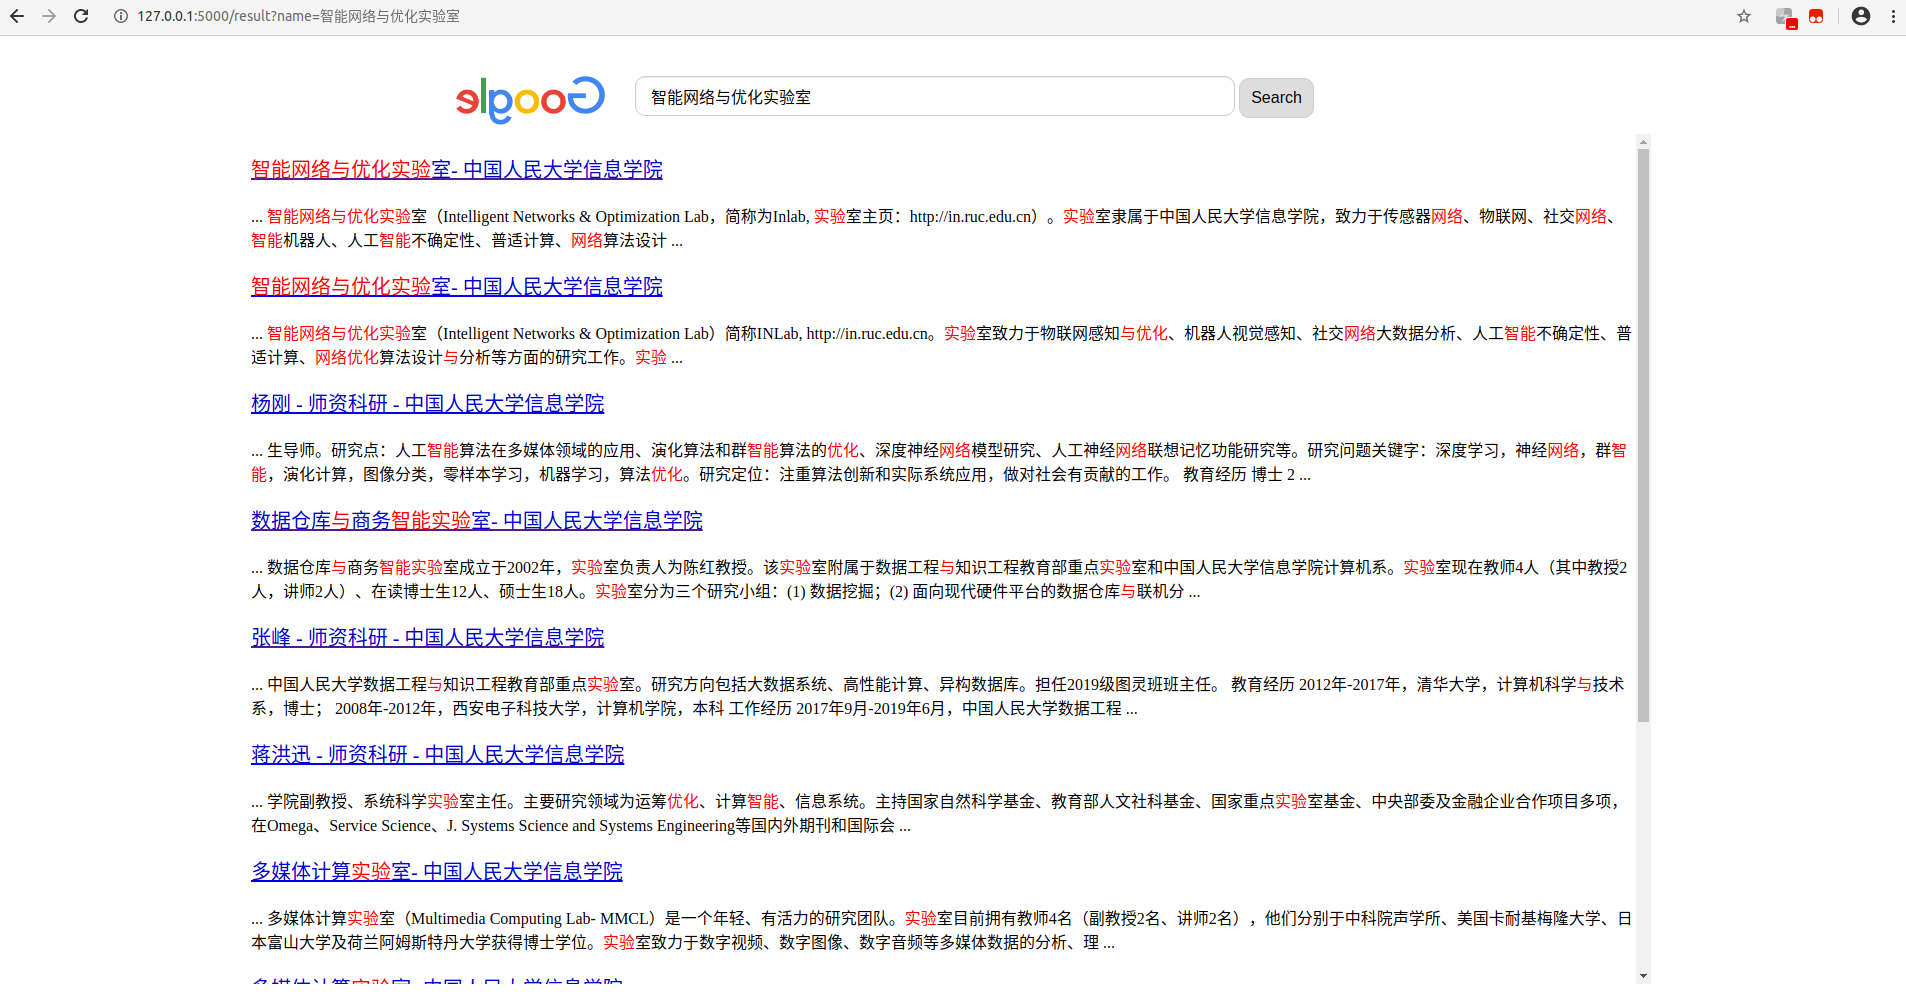
\includegraphics[width=0.6\textwidth, height=0.2\textheight]{lab.png}
	\end{center}

	Search for news:
	\begin{center}
		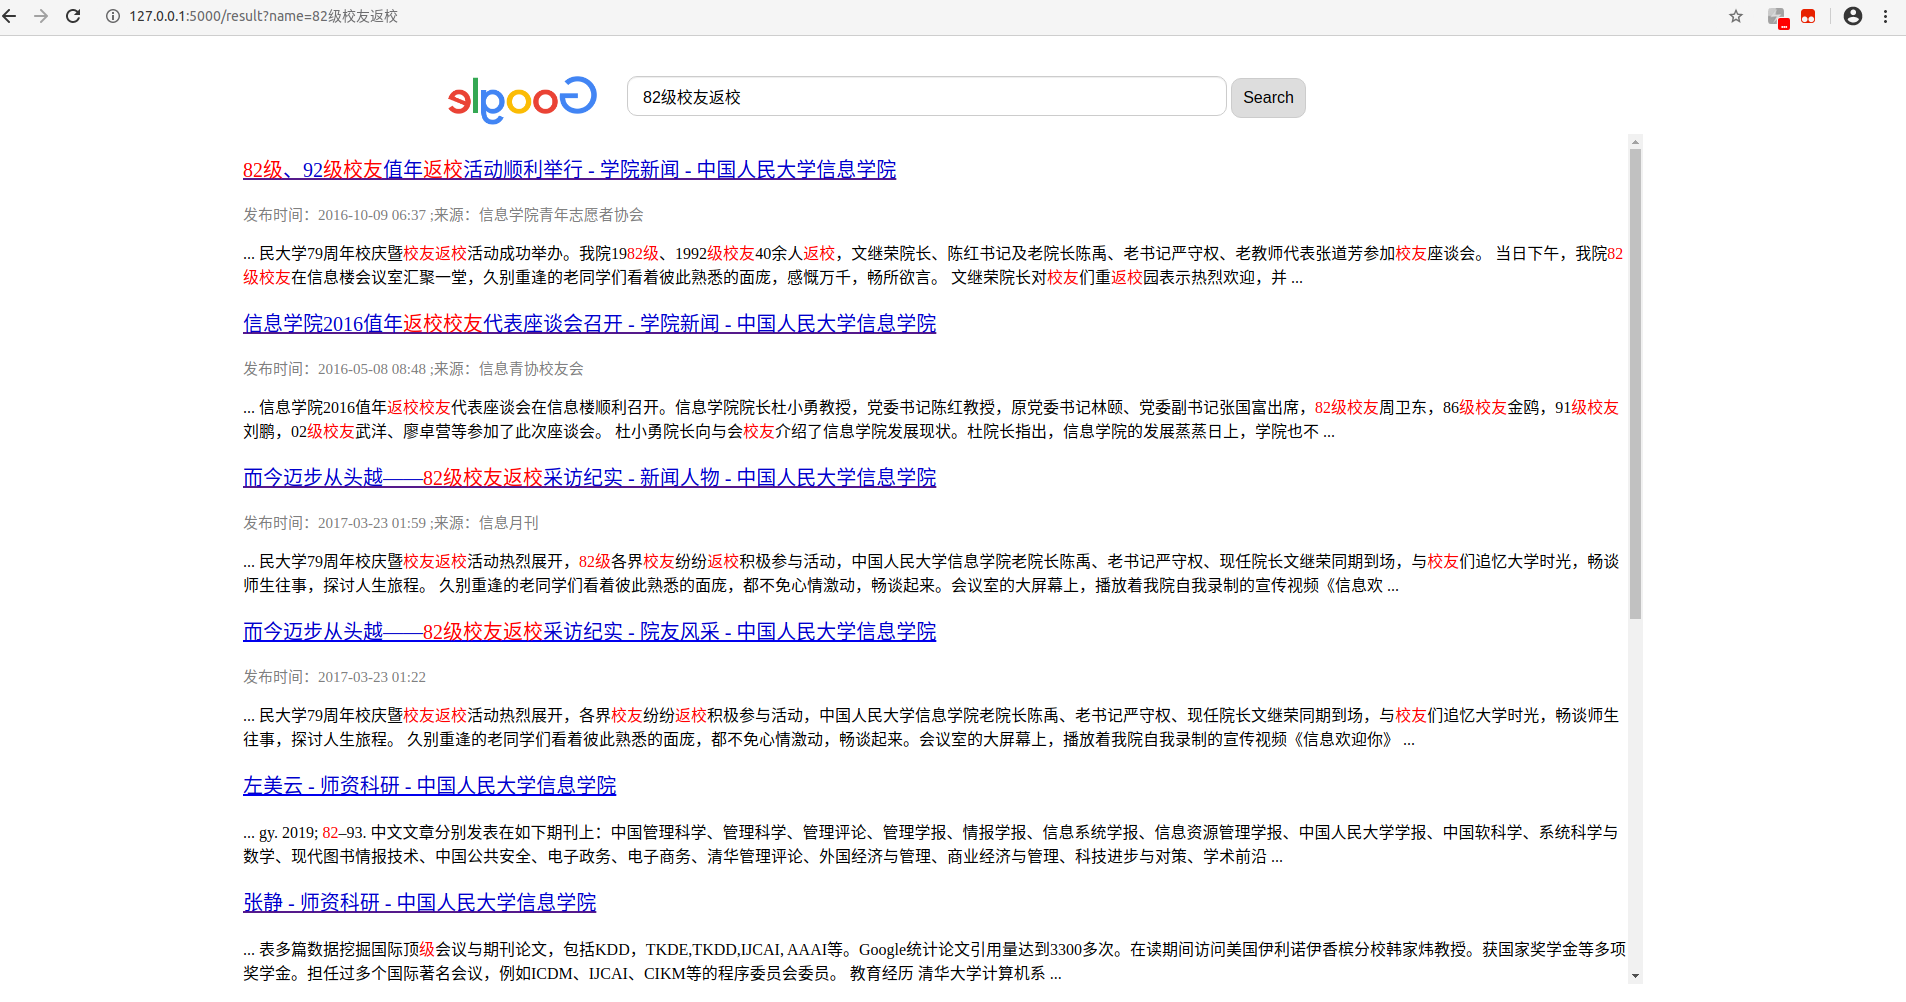
\includegraphics[width=0.6\textwidth, height=0.2\textheight]{82.png}
	\end{center}

\section{Summary}
	
	The elgooG Search Engine can present the relevant website for each query. I use C++ to make a crawler to download, use python to cut document into words and use inverted index to solve the query.

\section{How to build it in your computer}
	
	The search engine is based on Flask. You can download Flask by entering the command: 
	\lstset{numbers=left, %设置行号位置
		numberstyle=\small, %设置行号大小
		keywordstyle=\color{blue}, %设置关键字颜色
		commentstyle=\color[cmyk]{1,0,1,0}, %设置注释颜色
		frame=single, %设置边框格式
		escapeinside=``, %逃逸字符(1左面的键),用于显示中文
		%breaklines, %自动折行
		extendedchars=false, %解决代码跨页时,章节标题,页眉等汉字不显示的问题
		aboveskip=1em, %设置边距
		tabsize=4, %设置tab空格数
		showspaces=false %不显示空格
		language = bash
	}
\begin{lstlisting}
~$ pip3 install flask
\end{lstlisting}
	in terminal.
	
	If you want to make the search engine work, you should enter the command below in the path $YourPathToEngine/SearchEngine/UI/mywebapp/$ :
\begin{lstlisting}
~$ flask run
\end{lstlisting}
	
	Then terminal will show the local url in your computer, like the picture below:
	\begin{center}
		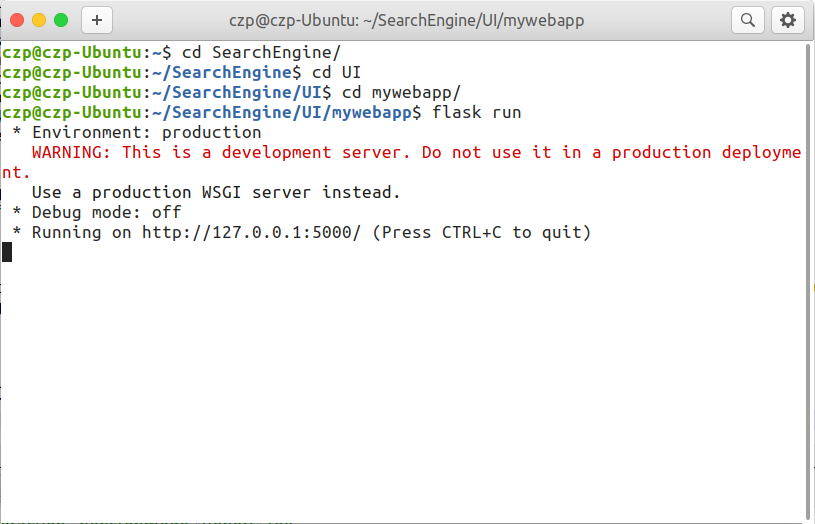
\includegraphics[width=0.4\textwidth, height=0.15\textheight]{terminal.png}
	\end{center}

	You can start the engine by entering the url into your browser.

\end{document}
